\documentclass[a4paper,12pt]{article}

\usepackage[spanish]{babel}
\usepackage[utf8]{inputenc}
\usepackage[T1]{fontenc}
\usepackage[utf8]{inputenc}
\usepackage{makeidx}
\usepackage{graphicx}
\usepackage{lmodern}
\usepackage{kpfonts}
\usepackage[left=2cm,right=2cm,top=2cm,bottom=2cm]{geometry}
\usepackage{amsmath,amsfonts,amssymb}
\usepackage{hyperref}
\hypersetup{
    colorlinks=true,
    linkcolor=cyan,
    filecolor=magenta,      
    urlcolor=blue,
    pdftitle={titulo},
    pdfpagemode=FullScreen,
    }
\urlstyle{same}

\title{Parcial 2}

\begin{document}

\begin{center}
\par 
\includegraphics[scale=1]{USB} \par
Universidad Simon Bolivar \\ Curso: CI4325 / Interfaces con el Usuario \\ Trimestre: Enero-Marzo, 2024 \\ Profesor: Franco Gabriel Nori Gonzalez \\ Estudiante: Junior Miguel Lara Torres - Carnet: 17-10303 \\
\end{center}

\begin{center}
Examen 2 (15\%)
\end{center}

\begin{itemize}

\item (7,5 puntos) Diseñe un prototipo que contenga al menos 10 de los siguientes patrones de diseño de interfaces:

\begin{itemize}
\item Presentación, búsqueda y navegación.
\item Ayuda multinivel.
\item Ventanas modales.
\item Menús grandes.
\item Plantillas o marcos visuales.
\item Alineación derecha o izquierda.
\item Balance diagonal.
\item Activación adaptativa.
\item Grilla de miniaturas.
\item Filas ralladas.
\item Paginación.
\item Cancelabilidad.
\item Pistas de entradas.
\item Mensajes de error de página.
\item Navegación de fondo.
\item Miniaturas con texto en lista.
\item Bordes generosos.
\end{itemize}

Nota: deberá listar cada uno de los patrones de diseño utilizados en su prototipo.

\newpage

EL prototipo se realizó en la plataforma figma.

\textit{\textbf{Todas las vistas: }} \href{https://www.figma.com/file/C2ED1xTr9Cfrh11yfhRsQ3/Examen2_Interfaces?type=design&node-id=0%3A1&mode=design&t=bNsMEHtXuUzC87qG-1}{Enlace a figma}

Para el prototipo creado tenemos los siguientes patrones de diseño:
\begin{enumerate}
\item Presentación, búsqueda y navegación.
\item Ventanas modales.
\item Menús grandes.
\item Plantillas o marcos visuales.
\item Activación adaptativa.
\item Grilla de miniaturas. (No del todo)
\item Filas ralladas.
\item Paginación.
\item Cancelabilidad.
\item Navegación de fondo.
\item Miniaturas con texto en lista.
\item Bordes generosos.
\item Pistas de entradas
\end{enumerate}

En las siguientes paginas se explican cada vista: 

\par 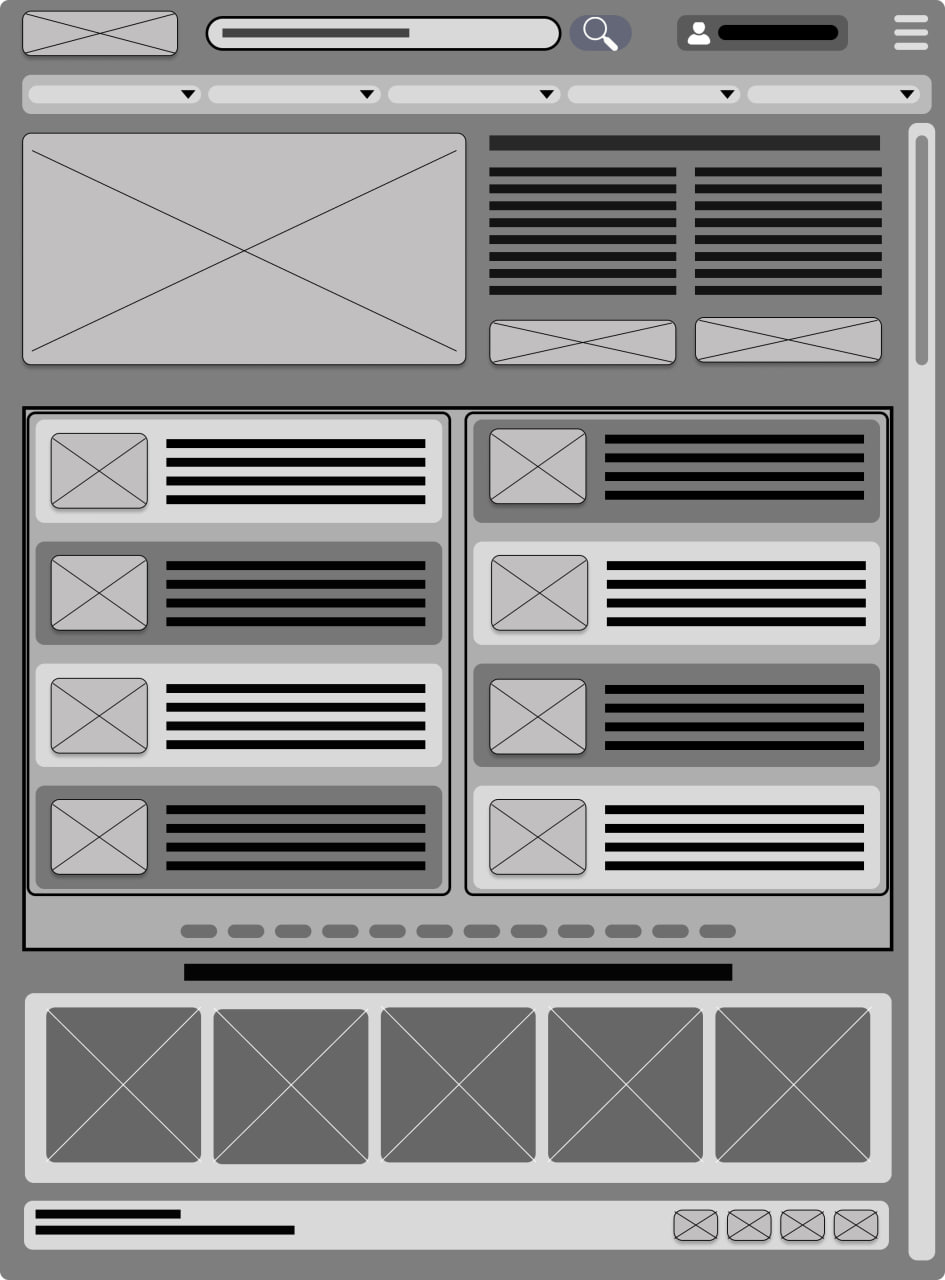
\includegraphics[scale=0.85]{m1} \par

Esta es la pagina principal donde se muestra el unico panel existente todo a borde generoso, una presentacion, menus, seccion de cuadriculas, un buscador, miniaturas con textos, una paginacion y un carrusel de multimedia, al final un footer respectivo.

\par 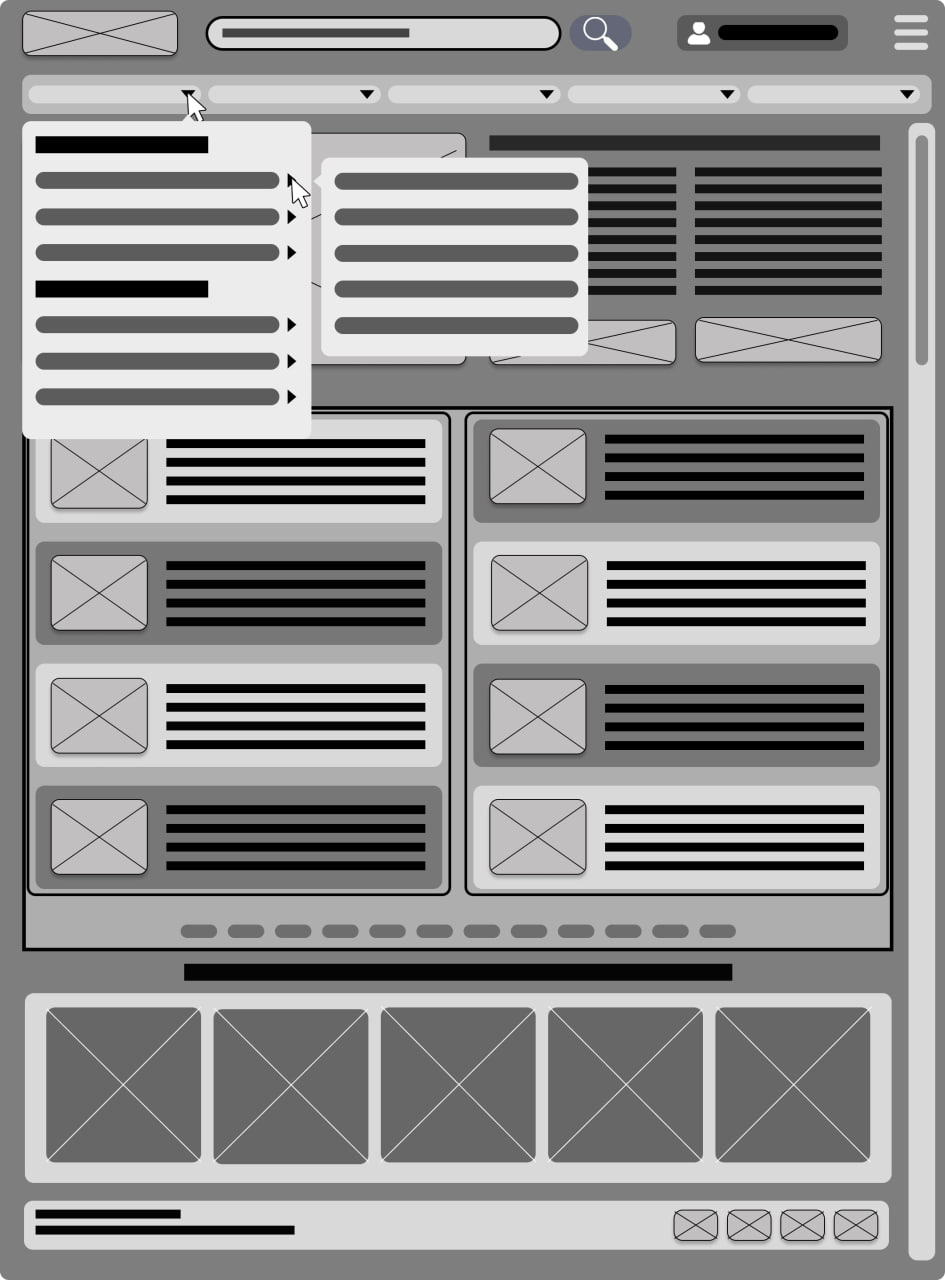
\includegraphics[scale=0.85]{m2} \par

Acá se muestra el despliegue de menus, que a primeras vistas se hizo pequeño pero se asume que habrán muchas opciones allí. Como se observa esta cuenta con navegacion de fondo al mismo tiempo.

\par 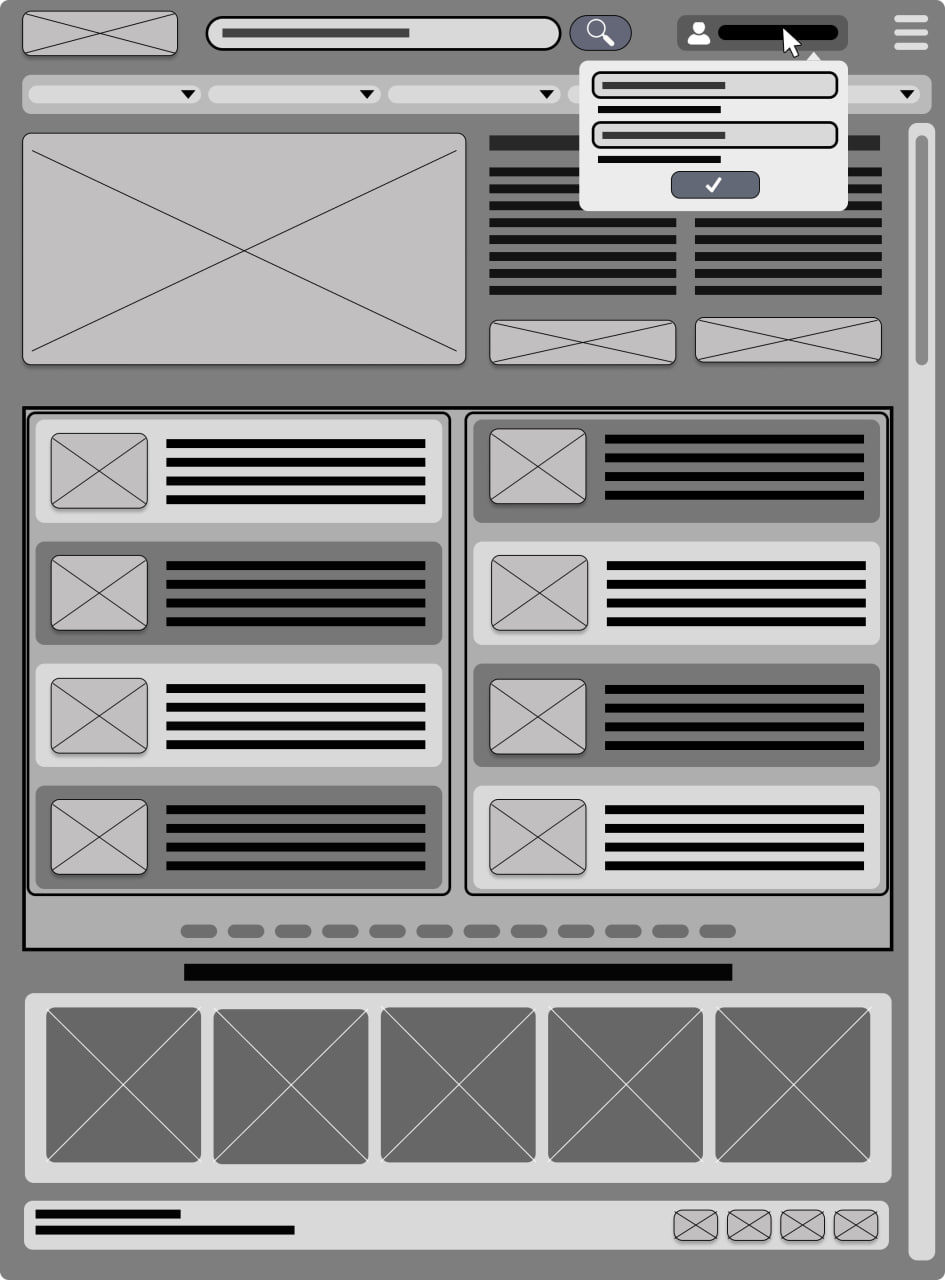
\includegraphics[scale=0.85]{m3} \par

Aqui ya se muestra la primera ventana modal del prototipo para el login de u usuario en esencia bajo pistas de entradas.

\par 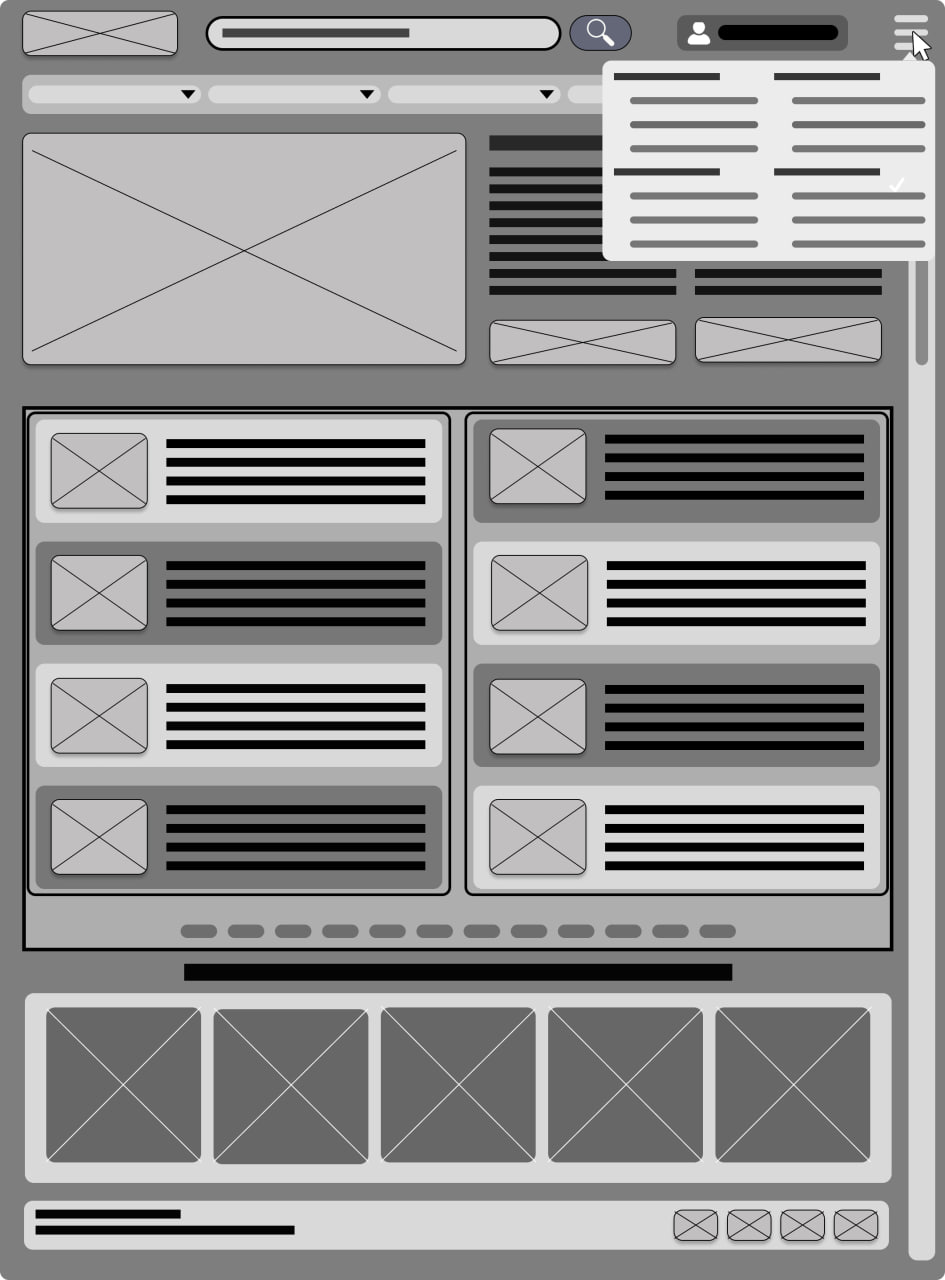
\includegraphics[scale=0.85]{m4} \par

Esta vista muestra el menu de opciones adicionales/configuraciones variadas en un formato ámplio. A todas estas, se puede agregar un mensaje de error de pagina al momento de realizar una busqueda erronea o al momento de no encontrar un match.

\par 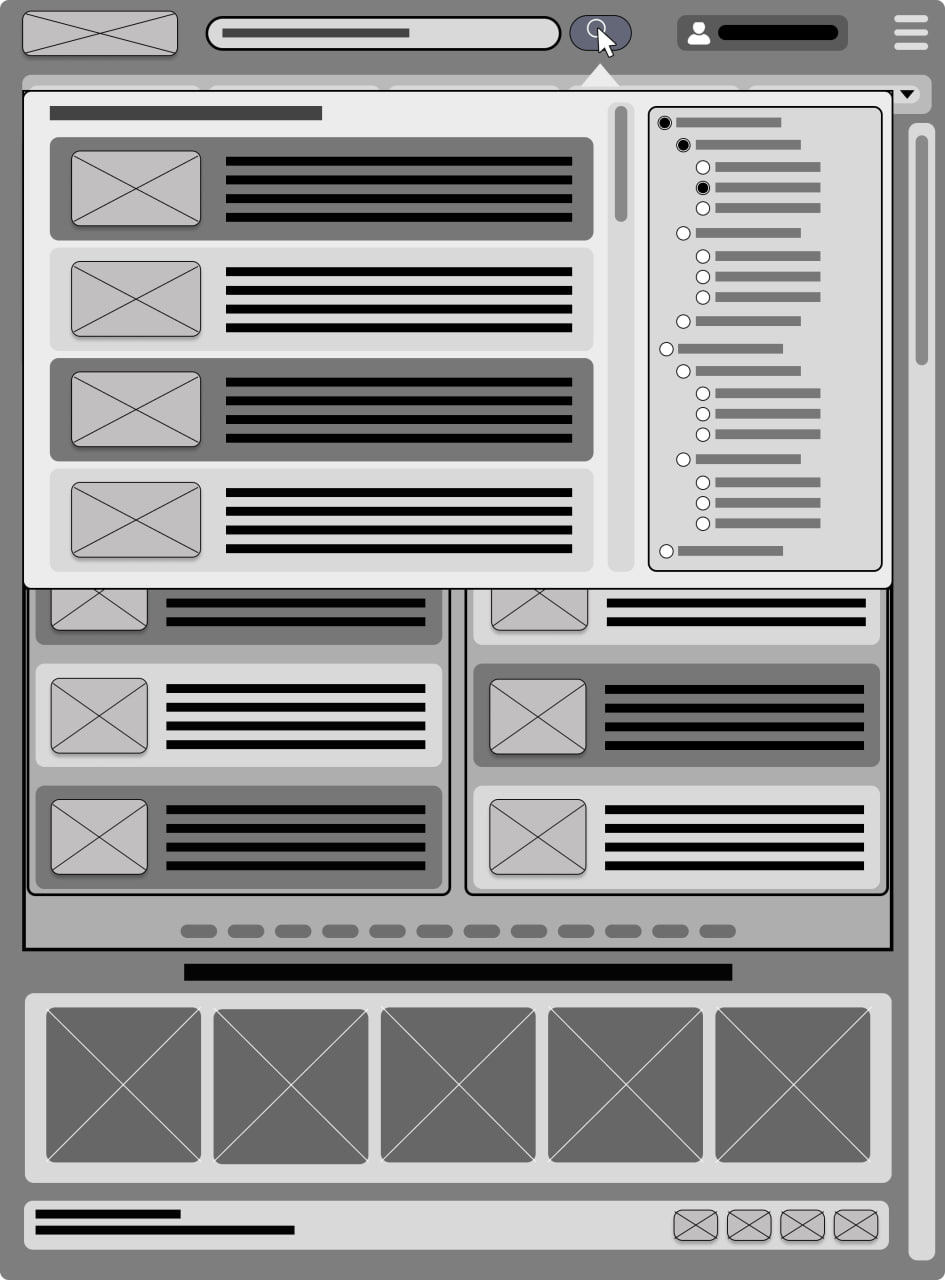
\includegraphics[scale=0.85]{m5} \par

El despliegue del buscador es por ventana modales que incluye filas ralladas y a su vez miniaturas con texto. Esta ventana dicionalmente cuenta con una seccion de filtros bajo el patrón de activación adaptativa. 

\par 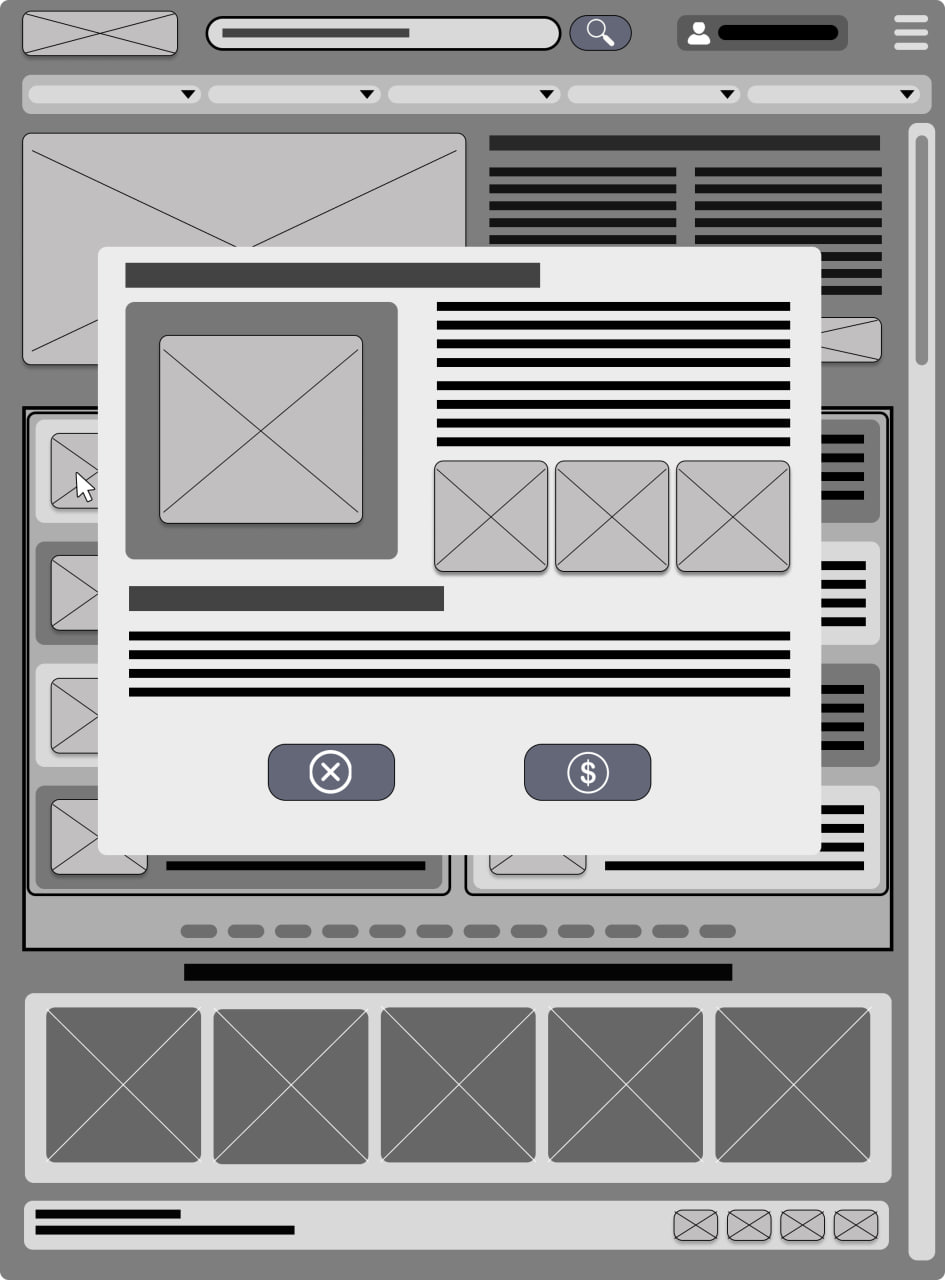
\includegraphics[scale=0.85]{m6} \par

Finalmente, se tiene las ventanas modales al dar click por medio del buscador o de la muestra en página principal de los productos, esta cuenta con un formato/plantilla/marco que nunca cambia, solo cambia la informacion presentada al usuario, respectivamente posee cancelabilidad.

\item (7,5 puntos) Sobre el prototipo diseñado establezca (de manera gráfica) elementos que estén relacionados con al menos 5 patrones de comportamiento. Elija sobre los siguientes patrones:

\begin{itemize}
\item Exploración segura.
\item Gratificación instantánea.
\item Cambios en el medio de la corriente.
\item Opciones diferidas.
\item Construcción incremental.
\item Microbreaks.
\item Memoria futura.
\item Repetición simplificada.
\item Solo teclado.
\item Consejo de otras personas.
\item Recomendaciones personales.
\end{itemize}

Nota: deberá listar y justificar cada uno de los patrones de comportamiento utilizados en su prototipo.

\begin{enumerate}
\item Exploración segura.\\
	La navegación segura se tiene dado que no existe mucha complejidad en el prototipo mostrado. Al momento de realizar una busqueda de un item o seleccionar uno existente a plena vista se muestra la informacion del mismo. No existen consecuencias mayores dado la simplicidad del prototipo.
	
\item Gratificación instantánea.\\
	Esto no esta presente los mockups pero puedo decir que es un detalle de implementacion que se tomará en cuenta, seria al momento de logearse u registrarse mostrará un aviso satisfactorio al usuario, al momento de realizar una búsqueda de algún item, si existen resultado favorables se mostrará con un aviso, al momento de finalizar una compra del item también.

\item Cambios en el medio de la corriente.\\
	Tenemos al momento de seleccionar un item de la lista bien sea por buscador o por plena vista en página principal se tiene la opcion de cambiar su opción mediante la cancelabilidad de su elección. 

\item Microbreaks.\\
	El proceso de búsqueda y selección de items no requiere un contrador de tiempo, asi que el usuario puede continuar cuando guste. Al momento de iniciar seccion, el usuario puede llenar sus datos y darle a iniciar seccion cuando guste.

\item Consejo de otras personas.\\
	Este apartado no se refleja en los mockups pero dado que este propotipo sigue la idea de un pagina que proporciona publicidad de items a los usuario en general, entonces se requiere que el cliente/usuario de su opinion y consejo de los productos bajo una calificacion.

\item Recomendaciones personales.\\
	Al igual que el patrón anterior, se debe dejar una caja de comentarios para indicar si la recomendacion del item es buena, regular o pésima en tal caso.

\end{enumerate}

\end{itemize}
\end{document}